%==============================================================================
\chapter{Modelo neural recursivo}\label{modeloneuralrecursivo}
%==============================================================================

Neste capítulo será explicado um dos modelos criados para resolver o problema de \ac{pos} Tagging. Para isso, vamos falar primeiramente quais são os pré-processamentos feitos; depois vamos definir a arquitetura do modelo; explicar o algoritmo de treinamento e de predição; e por fim, comentar sobre a implementação do modelo.

Com a intuição de simplificar o entendimento, já definimos variáveis que serão utilizadas no método de aprendizagem. Elas podem ser encontradas na \autoref{tab:variaveisdesenvolvimento}.
\begin{table}[!htb]
\caption{Notação utilizada para o modelo neural recursivo} \label{tab:variaveisdesenvolvimento}
\begin{center}
\begin{tabular}{P{1cm}m{13.0cm}}
  \toprule
  $m$   & número de exemplos de treinamento \\
  $d$		& dimensão das palavras e etiquetas vetorizadas \\
  $t$   & tamanho da janela de palavras e de classes \\
  $B$   & tamanho do \textit{beam} \\
  $J_p$ & janela de palavras \\
  $J_c$ & janela de classes (ou de etiquetas) \\
  $J_{c_b}$ & $b$-ésima janela de etiquetas, onde $0 \leq b < 0$ \\
  $S_n$  & $n$-ésima sentença \\
  $s_b$ & $b$-ésima sequência de palavras e etiquetas \\
  $p_b$ & $b$-ésimo vetor de probabilidades \\
  $M_b$ & $b$-ésima matriz de predição \\
  $M_{i,j}$ & elemento da linha $i$ e coluna $j$ da matriz de predição \\
  $h_{dim}$ & número de neurônios na camada oculta \\
  $\omega$	& conjunto de palavras \\
  $\gamma$  & conjunto de classes gramaticais \\
  $c_i$   & i-ésima classe gramatical da sentença, onde $c \in \gamma$ e $0 \leq i < |S_n|$ \\ 
  $w_i$   & i-ésima palavra da sentença, onde $w \in \omega$ e $0 \leq i < |S_n|$ \\
  $\imath(x)$  & função que retorna o índice da palavra ou classe $x$ \\
  $c_i^t$  & sequência de classes que começa em $i$ e termina em $t$ \\
  $w_i^t$  & sequência de palavras que começa em $i$ e termina em $t$ \\
  $V_i$		& vetor centrado em $i$ com os índices das $t$ palavras concatenados \\
  $I_t$ & matriz de dimensão $t \times t$ com $1$s na diagonal secundária \\
  $Q$	&	conjunto com os índices das palavras já classificadas \\
  $P$ & Fila de prioridades de tamanho $B$ \\
  \bottomrule
\end{tabular}
\end{center}
\end{table}

Optamos por criar um modelo neural recursivo pois acreditamos que uma rede neural recursiva pode ajudar a classificar corretamente as palavras devido ao fato de haver um contexto de etiquetas. Esse contexto é variável, e portanto, também acreditamos que a rede neural recursiva pode lidar com longa dependência.


\section{Pré-processamento}

Para cada sentença $S_n$ nós criamos uma janela com $t$ índices das palavras $\{\imath(w_1), ..., \imath(w_t)\}$, para computar a n-ésima palavra, é centralizada a janela em $n$ e concatena-se todos os índices das palavras da metade à esquerda e da metade à direita em um novo vetor $V_n$ de dimensão $t \times 1$. A \autoref{eq:janeladevets} demonstra isso.

\begin{equation} \label{eq:janeladevets}
V_n = \big\{ \imath(w_{n - \lfloor t/2 \rfloor}), ..., \imath(w_n), ..., \imath(w_{n + \lfloor t/2 \rfloor}) \big\}
\end{equation}

Para palavras no começo da sentença, as $\lfloor t/2 \rfloor$ palavras à esquerda não existem. Para contornar esse problema nós preenchemos esses espaços com um símbolo (\textit{token}) especial. O mesmo ocorre para palavras no fim da sentença. 

Nosso modelo contou com quatros \textit{tokens} especiais listados abaixos

\begin{itemize}
\item \texttt{<mask>}: Para as extremidades da janela de palavras e da janela de etiquetas.
\item \texttt{<unknown>}: Para palavras raras ou desconhecidas.
\item \texttt{<padding\_prefix>}: Para completar o vetor de prefixos.
\item \texttt{<padding\_suffix>}: Para completar o vetor de sufixos.
\end{itemize}

Consideramos uma palavra como sendo rara quando a quantidade de ocorrências dela no treinamento é menor que um hiperparâmetro determinado no momento da compilação.


\section{Arquitetura} \label{sec:arquiteturarecursiva}

A arquitetura do modelo neural recursivo implementado pode ser vista na \autoref{fig:recursivemodel}.

\begin{figure}[!htb]
    \caption{Arquitetura da rede neural recursiva}\label{fig:recursivemodel}
    \begin{center}
        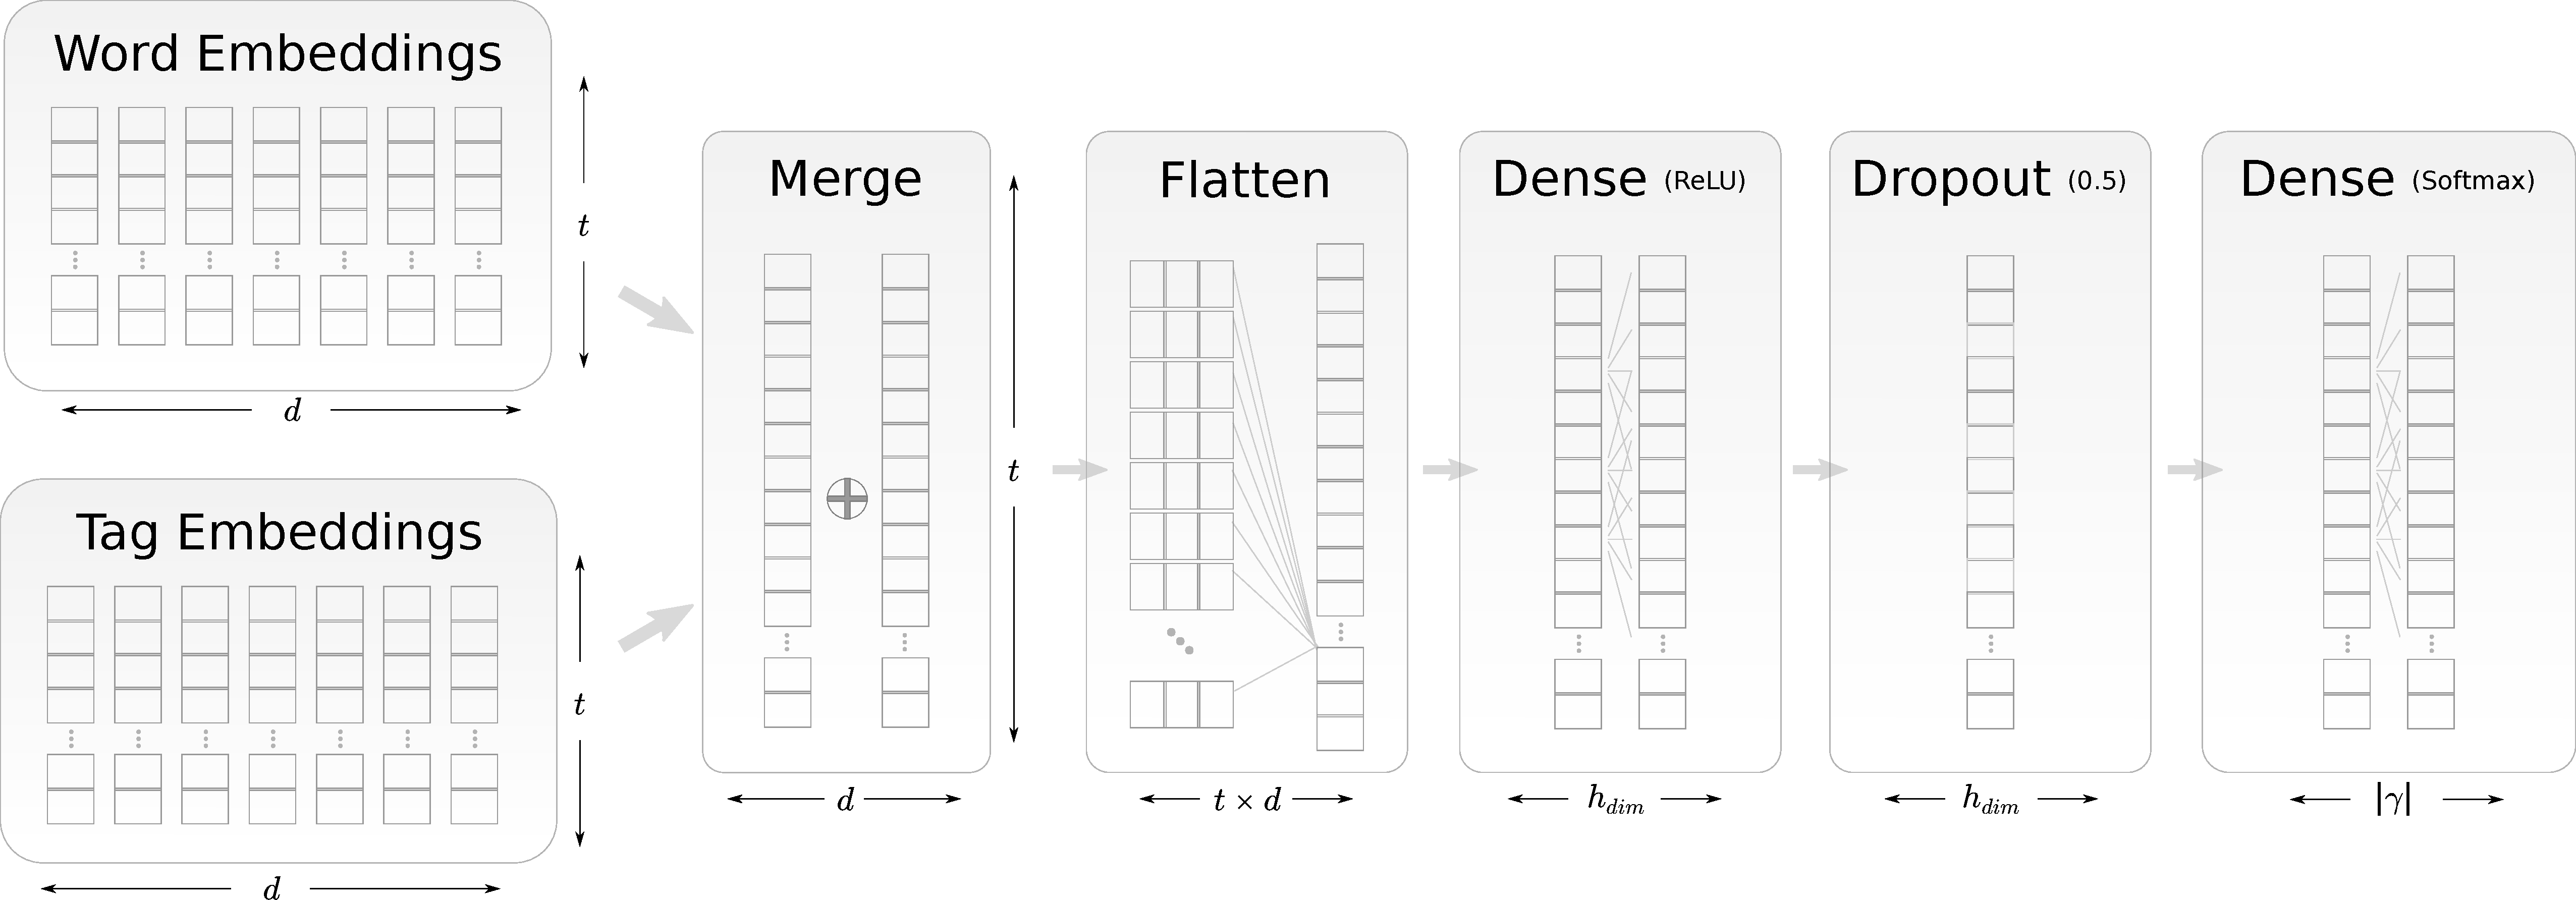
\includegraphics[scale=0.19]{img/recursive_model_horizontal.pdf}
    \end{center}
\end{figure}

Como entrada da rede é passado a janela de palavras e uma janela de \textit{tags} (etiquetas) das palavras já etiquetadas. A janela de etiquetas é passada para a camada \textit{Tag Embeddings} e a janela de palavras é passada a camada \textit{Word Embeddings}. Fizemos uma composição através de uma operação de soma dos vetores das \textit{tags} com os vetores das palavras. Após calcular a composição dos vetores de palavras com os vetores das etiquetas, nós concatenamos todos os vetores dentro da janela e passamos para a próxima camada. Aplicamos esses vetores concatenados a uma camada totalmente conectada (\textit{Fully connected} ou \textit{Dense}) com a função de ativação \ac{relu} \autoref{eq:relueq}. Aplicamos a saída da camada densa um \textit{dropout}, que é responsável pela regularização da rede. No fim adicionamos mais uma camada densa com um \textit{softmax} (\autoref{eq:softmaxeq}) como ativação para nos dar uma probabilidade normalizada.

\begin{equation}\label{eq:relueq}
ReLU(x) = max(0, x)
\end{equation}
\begin{equation}\label{eq:softmaxeq}
softmax(x) = \frac{e^{x_j}}{\sum_{k=1}^{n} e^{x_k}}, \quad \mbox{para } j = 1, ..., n
\end{equation}


\subsection{Embeddings: camada de vetores de palavras e etiquetas}

Essa camada é responsável por treinar os vetores de palavras. Seu funcionamento é bem simples: fizemos o \textit{Backpropagation} até a camada de entrada, desse modo, podemos transformar índices para vetores usando uma tabela de pesquisa com uma função de mapeamento de um para um. 

Como por exemplo, pode ser feita a transformação de \texttt{[[2, 3], [5, 7]]} em \texttt{[[[0.1, 0.2], [0.25, 0.85]], [[0.53, 0.39], [0.22, 0.84]]]}. Ou seja, damos como entrada uma matriz com formato $m \times t$ e é retornado uma matriz com formato $m \times t \times d$. Como opção, podemos atribuir os pesos de cada índice (ou seja, o vetor da palavra) no momento da compilação e ajustá-los conforme o treinamento. 

A camada \textit{Word Embeddings} foi dividida em quatro partes: Uma parte é reponsável por atribuir os vetores distribuídos de palavras; outra parte trata de prefixos e sufixos; e ainda há uma parte que trata de capitalização. Para cada uma dessas partes foi atribuído os pesos no momento da compilação, desse modo o vetor de cada \textit{feature} fica ajustado à tarefa de \ac{pos} Tagging.



\subsection{Merge: camada de composição}

É responsável por juntar os dois submodelos: modelo de vetores de palavras e de vetores de etiquetas. Isso é feito através de uma função de composição. No nosso caso foi usado uma função de soma. Desse modo, a matriz resultante continua com o mesmo formato. 

Nessa camada, estamos combinando características do vetor de uma palavra com o respectivo vetor de uma classe gramatical associada a essa palavra.


\subsection{Flatten: camada de concatenação}

Simplesmente faz a concatenação das linhas da matriz de entrada. Ou seja, vai transformar a matriz com formato $m \times t \times d$ em uma matriz de duas dimensões com formato $m \times t*d$.


\subsection{Dense: camada totalmente conectada}

É uma simples camada neural onde cada neurônio da camada atual é ligado a todos os neurônios da próxima camada. Portanto, o formato da matriz resultante é $m \times h_{dim}$. 

A primeira camada Dense é aplicada a função de ativação \ac{relu} descrita na \autoref{eq:relueq}. A escolha dessa função de ativação foi feita de modo empírico.

Já na segunda camada Dense é aplicada a função de ativação \textit{softmax} para nos dar probabilidades normalizadas.

\subsection{Dropout: camada de regularização}

\textit{Dropout} é uma técnica introduzida em \cite{srivastava2014dropout} para previnir \textit{overfitting} nas redes neurais. Quando uma rede neural é treinada, um neurônio tem probabilidade $p$ (nesse caso $p=0.5$) de ser ignorado durante a computação do \textit{forward propagation} e do \textit{Backpropagation}. A \autoref{fig:dropout} demonstra essa técnica. 

\begin{figure}[!htb]
    \caption{Exemplo de \textit{Dropout}}\label{fig:dropout}
    \begin{center}
        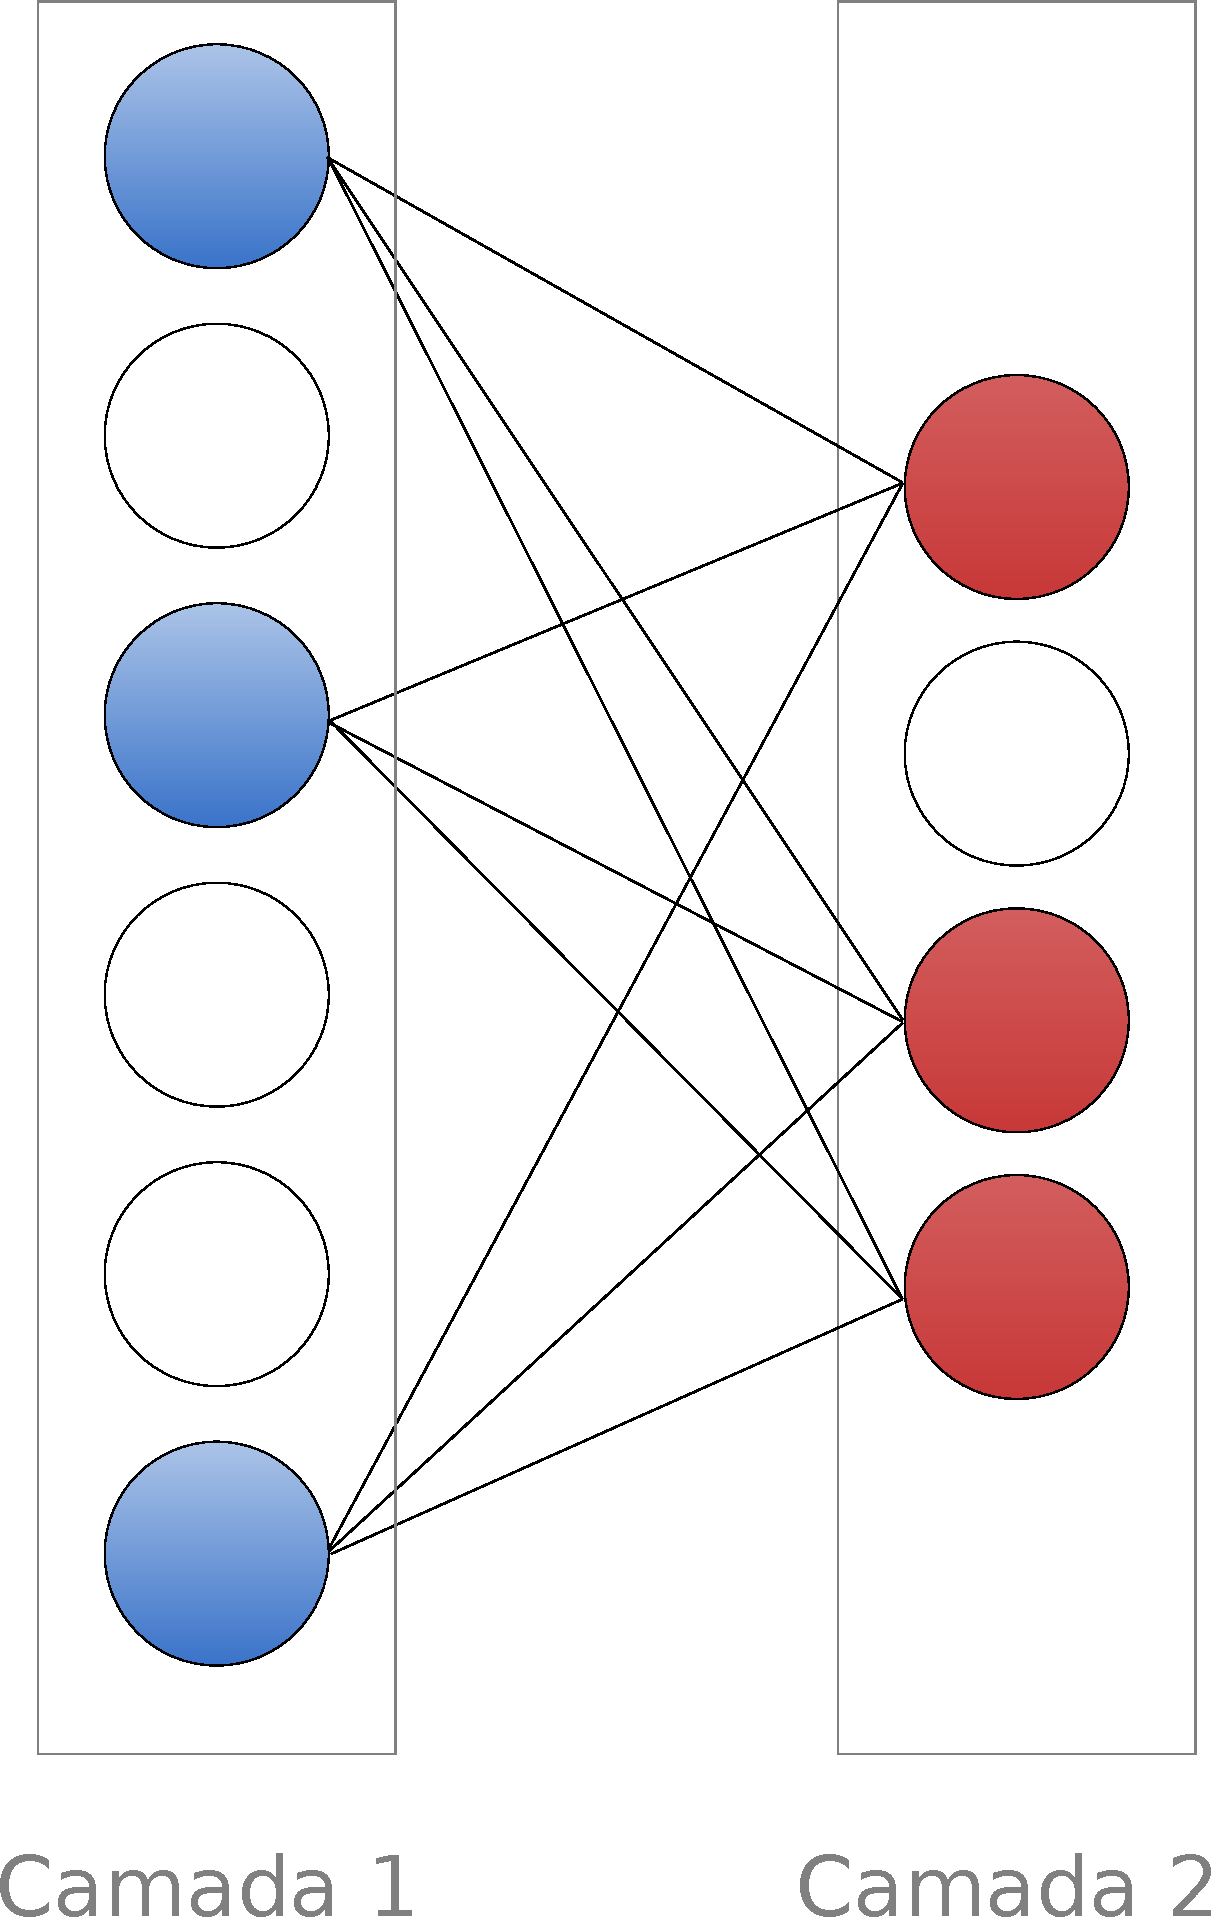
\includegraphics[scale=0.12]{img/dropout.pdf}
    \end{center}
\end{figure}



\section{Treinamento}

Nosso modelo recursivo baseia-se em escolher as palavras mais fáceis para serem etiquetadas primeiro. Essa heurística também é utilizada em \cite{shen2007guided} para o algoritmo de inferência. 

Uma palavra é caracterizada como mais fácil quando a saída da rede neural para uma de suas etiquetas for a maior entre todas na sentença. Por exemplo, suponhamos que temos a sentença: \texttt{Computação é um curso legal!}, e que temos apenas 3 etiquetas possíveis: \texttt{substantivo; adjetivo; verbo}. Quando jogamos cada palavra na rede neural, temos a seguinte matriz mostrada na \autoref{tab:exemplodeetiquetacao}.


\begin{table}[!htb]
\caption{Exemplo de etiquetação} \label{tab:exemplodeetiquetacao}
\begin{center}
\begin{tabular}{c|c|c|c}
  \toprule
  Palavra/Etiqueta & substantivo & adjetivo & verbo \\
  \midrule
  Computação & 0.6 & 0.2 & 0.2 \\
  \midrule
  é          & 0.7 & 0.2 & 0.1 \\
  \midrule
  um         & 0.1 & 0.6 & 0.3 \\
  \midrule
  curso      & \textbf{0.8} & 0.1 & 0.1 \\
  \midrule
  legal      & 0.4 & 0.4 & 0.2 \\
  \midrule
  !          & 0.5 & 0.4 & 0.1 \\
  \bottomrule
\end{tabular}
\end{center}
\end{table}

Nesse caso, a palavra mais provável é \texttt{curso}, pois a etiqueta \texttt{substantivo} tem a maior probabilidade entre todas as etiquetas de todas as palavras. Formalmente, a palavra mais provável pode ser obtida através da \autoref{eq:maisprovavel}.

\begin{equation}\label{eq:maisprovavel}
\argmax_{i}\Big(\max_{0 \leq j \leq |\gamma|}(M_{i,j})\Big)
\end{equation}

Treinamos o modelo por sentença, onde levamos em consideração duas entradas para a rede neural: A janela de palavras $J_p$ e a janela de etiquetas $J_c$ inicializada com um valor especial de ``etiqueta desconhecida''. Além disso, inicializamos o conjunto $Q$ de palavras já etiquetadas com o valor $\emptyset$. A cada passo do algoritmo, obtemos a palavra mais provável que ainda não foi etiquetada e sua respectiva etiqueta serve de contexto para a próxima palavra a ser prevista. Esse contexto é colocado em cada vetor em que essa palavra estava associada na janela de etiquetas. O processo continua até que o tamanho do conjunto $Q$ seja igual o tamanho da sentença, ou seja, até que todas as palavras tenham sido classificadas.

Podemos representar o processo de obter a palavra mais provável que ainda não foi etiquetada através de uma modificação da \autoref{eq:maisprovavel}, mostrada abaixo na \autoref{eq:maisprovavelnaoetiquetada}.

\begin{equation}\label{eq:maisprovavelnaoetiquetada}
mp(M) = \argmax_{i \not \in Q}\Big(\max_{0 \leq j \leq |\gamma|}(M_{i,j})\Big)
\end{equation}

E o processo de atualizar o contexto para prever a próxima palavra é mostrado na \autoref{eq:atualizarcontexto}. Onde $c_x$ representa a etiqueta prevista, $x$ representa a entrada e $I_t$ representa uma matriz com $1$s na diagonal secundária com dimensão $t \times t$.

\begin{equation}\label{eq:atualizarcontexto}
J_c[mp(x)-\lfloor t/2 \rfloor:mp(x)+\lfloor t/2 \rfloor][I_t] = c_{mp(x)}
\end{equation}

O algoritmo \ref{algoritmotreinamento} realiza todo esse processo.

\begin{algorithm}[!htb]
\caption{Algoritmo de Treinamento} \label{algoritmotreinamento}
\begin{algorithmic}[1]
\Procedure{Treinamento}{}
  \State dado um conjunto de treinamento $\{X, Y\}$
  \For{cada sentença $S_n$ em $\{X, Y\}$}
    \State $J_p = $ janela de palavras da sentença $S_n$
    \State $J_c[:] = $ etiqueta desconhecida 
    \State $Q = \{\}$ 
    \While{$Q.size < s_t.size$}
      \State $train\_on\_batch$([$J_p, J_c$], $Y_{S_n}$)
      \State $M = predict\_on\_batch$([$J_p, J_c$])
      \State palavra\_mais\_provável = $mp(M)$
      \State tag\_mais\_provável = $J_c$[palavra\_mais\_provável]
      \State $slice = \mbox{palavra\_mais\_provável}-\lfloor t/2 \rfloor:\mbox{palavra\_mais\_provável}+\lfloor t/2 \rfloor$
      \State $J_c[slice][I_t] = \mbox{tag\_mais\_provável}$
      \State $Q.add(\mbox{palavra\_mais\_provável})$
    \EndWhile
  \EndFor
\EndProcedure
\end{algorithmic}
\end{algorithm}


\subsection{Minimização da função de custo}

A função de custo utilizada nesse modelo foi a \textit{Categorical Cross-entropy} mostrada na \autoref{eq:categorial_crossentropy}, onde $y$ é o nosso conjunto de classes gramaticais, e $\hat{y}$ é a classe prevista pela rede. 

\begin{equation} \label{eq:categorial_crossentropy}
J(\theta) = - \frac{1}{m} \sum\limits_{i=1}^{m} \Big[ y_ilog(\hat{y}_i) + (1 - y_i)log(1 - \hat{y}_i) \Big]
\end{equation}

Para minimizar essa função de custo, nós utilizamos um otimizador de segunda ordem baseado no Gradiente Descendente chamado Adadelta \cite{Bengio-et-al-2015-Book}. O Adadelta leva em consideração informações de cada dimensão dos dados para atualizar a taxa de aprendizagem. Essa abordagem tem diversas vantagens:

\begin{itemize}
\item Taxa de aprendizagem dinâmica por dimensão.
\item Pequena quantidade computação por iteração.
\item Hiperparâmetros escolhidos não afetam tanto o resultado. 
\end{itemize}

A implementação do Adadelta utilizada foi a disponível na biblioteca Keras \cite{kerasframework}.



\subsection{Análise de complexidade temporal}\label{subsec:analisecomplexidade1}

A nossa implementação utilizou um simples vetor de \textit{flags} de tamanho igual ao da sentença como sendo o conjunto de palavras já etiquetadas $Q$. Desse modo, gastamos $O(1)$ para descobrir se uma palavra já foi classificada. 

Para cada palavra $w_i$ numa sentença $S_n$, treinamos a rede neural num $batch$ de tamanho $|S_n|$. Como a rede neural depende de parâmetros para a convergência, vamos impor um limite aproximado de $\theta((t*d*h_{dim})^3)$, que equivale a multiplicações de matriz dos vetores de palavras concatenados com a camada oculta. Além disso, fizemos $O(|S_n| * |\gamma|)$ iterações para buscar qual é a palavra mais provável. E por fim, atualizamos a janela de etiquetas fazendo $O(t)$ iterações.

Supondo que todas as sentenças tenham tamanhos iguais (e portanto $avg(S_i) = |S_n|$ para todo $0 \leq i < m $):
\begin{equation} \nonumber
O(|S_n| * ((t*d*h_{dim})^3 + (|S_n| * |\gamma|) + t))
\end{equation}

Como $t$ no pior dos casos é igual a $|S_n|$, temos:
\begin{align} 
O&(|S_n| * ((|S_n|*d*h_{dim})^3 + (|S_n| * |\gamma|) + |S_n|)) \nonumber \\
O&(|S_n|^4 * (d*h_{dim})^3 + |S_n|^2*(|\gamma| + 1)) \nonumber \\
O&(|S_n|^4 * (d*h_{dim})^3 + |S_n|^2*|\gamma|) \nonumber \\
O&(|S_n|^4 * (d*h_{dim})^3) \nonumber
\end{align}

Dentre essas variáveis, as únicas que não podemos controlar são $|S_n|$ e $|\gamma|$, porém $|\gamma|$ geralmente é um valor muito pequeno, e consequentemente, toda a computação recai sobre o tamanho da sentença. Com isso, podemos perceber que se o tamanho médio das sentenças for muito grande, então a computação vai ser demorada. 





\section{Predição}

Para classificar uma palavra, nós seguimos a ideia apresentada por \cite{shen2007guided} e utilizamos um \textit{beam search} sobre as classes mais prováveis da palavra mais provável (i.e. palavra mais fácil) em um determinado instante.

Inicializamos a janela de etiquetas com a etiqueta desconhecida e pegamos a primeira palavra mais provável e suas $B$ tags mais prováveis. Após fazer isso, inicializamos $B$ sequências para armazenar quais palavras foram etiquetadas e com quais tags elas foram etiquetadas. Inicializamos também a probabilidade de cada sequência $s_b$ com o valor $1$. E criamos uma lista de matrizes de predições $M_b$ para cada $0 \leq b < B$.

Para cada sequência, nós utilizamos suas etiquetas já previstas como contexto na rede neural para realizar uma nova predição. Criamos uma fila de prioridade truncada com tamanho $B$ para armazenar as próximas sequências. A prioridade da fila é a probabilidade da sequência vezes a probabilidade das etiquetas para a palavra mais provável. Após fazer isso, atualizamos nossas sequências e suas probabilidades para então voltar ao processo de predição para cada sequência. O processo termina quando todas as sequências estiverem completas, isso é, quando $\sum_{b=0}^{B}s_b.size = B*|S_n|$. 

O algoritmo \ref{algoritmopredicao} sumariza esse processo.

\begin{algorithm}[!htb]
\caption{Algoritmo de Predição} \label{algoritmopredicao}
\begin{algorithmic}[1]
\Procedure{Predição}{}
  \State dado um conjunto para ser etiquetado $\{X\}$
  \State dado o tamanho do \textit{beam} $B$
  \For{cada sentença $S_n \in X$}
    \State $J_p = $ janela de palavras da sentença $S_n$
    \State $J_{c_b}[:] = $ etiqueta desconhecida 
    \State $s_b[:] = []$
    \State $p_b[:] = 1$ 
    \State $M_b[:] = $ $predict\_on\_batch$([$J_p, J_{c_b}$])
    \State $P$ = PriorityQueue($beam\_size=B$)
    \State $P.push(M_b[:])$
    \While{$\sum_{b=0}^{B} s_b.size < B*|S_n|$}
      \State mais\_prováveis = $P.get\_items\_and\_pop()$
      \For{palavra\_mais\_provável, tag\_mais\_provável, $b \in$ mais\_prováveis}
        \State $slice = \mbox{palavra\_mais\_provável}-\lfloor t/2 \rfloor:\mbox{palavra\_mais\_provável}+\lfloor t/2 \rfloor$
        \State $J_{c_b}[slice][I_t] = \mbox{tag\_mais\_provável}$
        \State $p_b$ *= $M_b$[palavra\_mais\_provável][tag\_mais\_provável]
        \State $s_b.add$((palavra\_mais\_provável, tag\_mais\_provável))
        \State $M_b = predict\_on\_batch$([$J_p, J_{c_b}$])
      \EndFor
      \State próxima\_mais\_provável = $mp$($\max(M_b)$)
      \State probs = $zip$($M_b$[próxima\_mais\_provável, :], $p_b$)
      \For{probabilidade\_tag, probabilidade\_sentença $\in$ probs}
        \State nova\_prioridade = probabilidade\_tag * probabilidade\_sentença
        \State novo\_item = $M_b$[próxima\_mais\_provável]
        \State $P.push\_with\_priority$(novo\_item, nova\_prioridade)
      \EndFor 
      \State mais\_prováveis = $P.get\_items()$
      \State $swap$($s_b$, $s_b$[mais\_prováveis.$b$])
      \State $swap$($p_b$, $p_b$[mais\_prováveis.$b$])
    \EndWhile
  \EndFor
\EndProcedure
\end{algorithmic}
\end{algorithm}


Esse nosso algoritmo consegue usar contexto de palavras não vizinhas, desse modo espera-se resolver problemas de longa dependência.

Para entender melhor o funcionamento do algoritmo, sua execução está demonstrada na \autoref{fig:execpredicao}.

\begin{figure}[!htb]
    \caption{Exemplo de predição}\label{fig:execpredicao}
    \begin{center}
        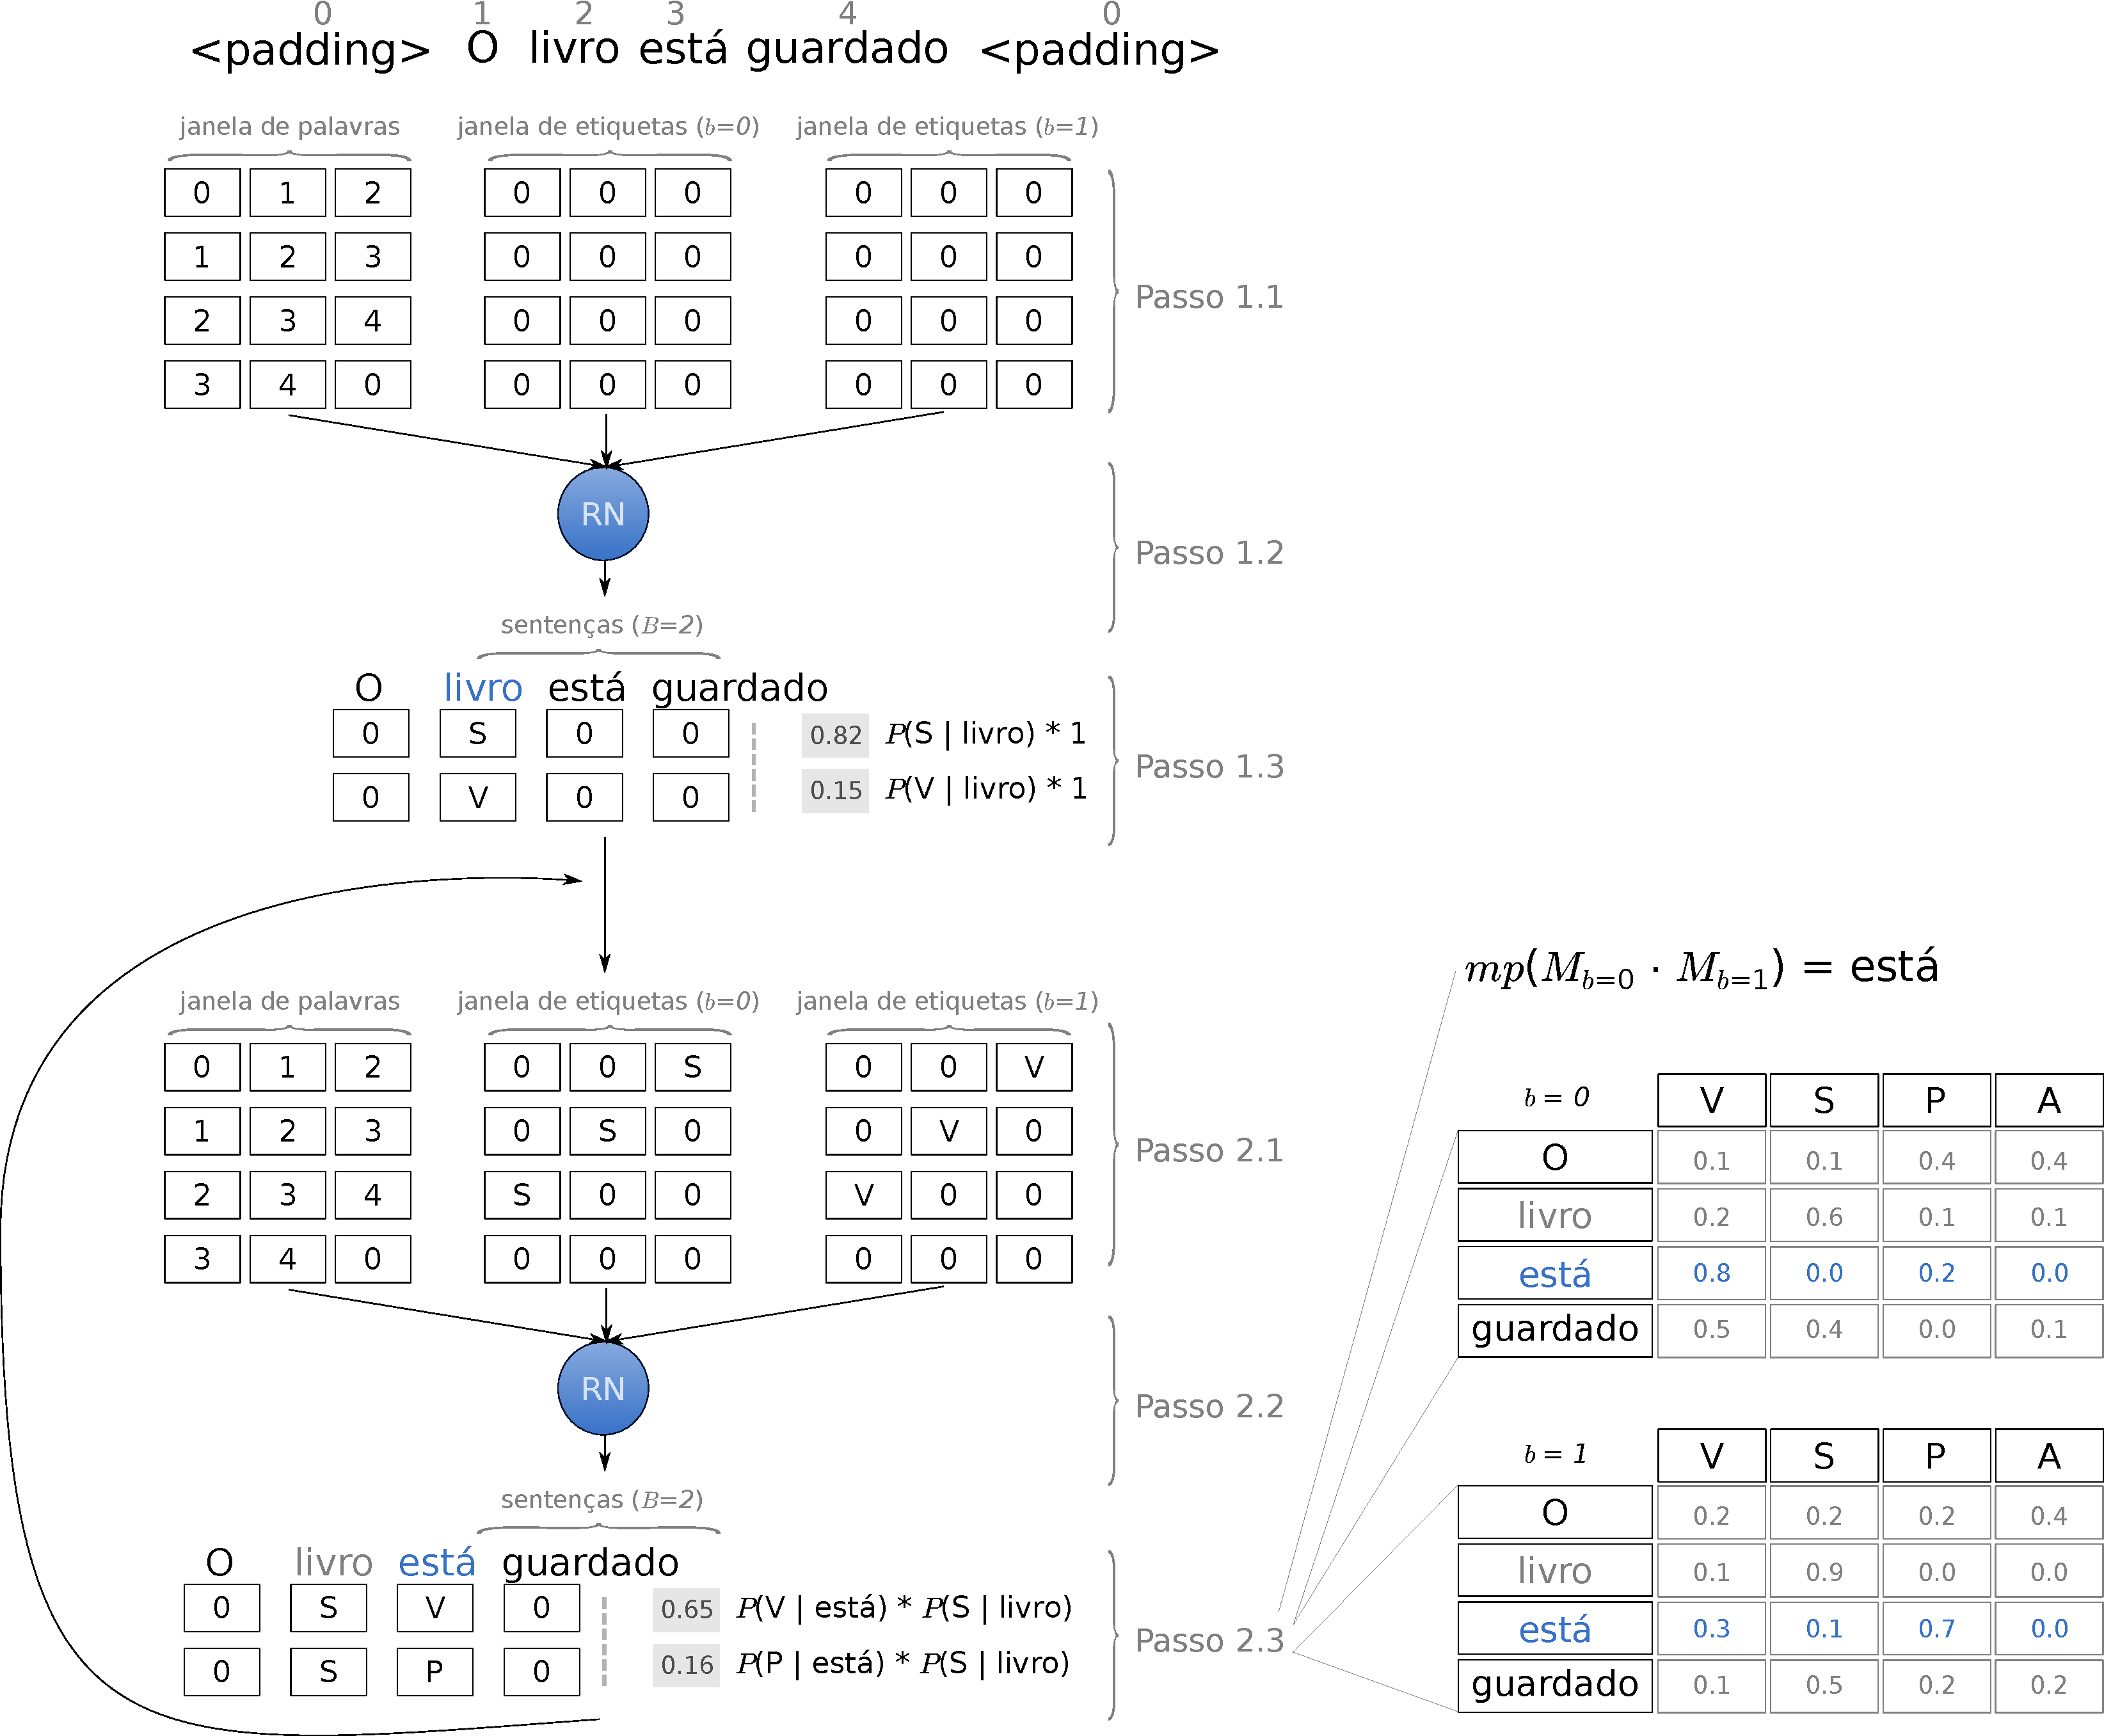
\includegraphics[scale=0.25]{img/algoritmodepredicao.pdf}
    \end{center}
\end{figure}

Realizamos dois passos do algoritmo na \autoref{fig:execpredicao}. Exemplificamos com uma sentença simples: ``O livro está guardado''. Utilizamos $t = 3$ e identificamos cada palavra na sentença pelo seu índice. Perceba que foi adicionado um símbolo especial de preenchimento chamado ``<padding>'' à esquerda e à direita da sentença. Nesse exemplo, definimos $B = 2$ para simplificar a visualização. O círculo azul representa a rede neural já treinada de acordo com a seção anterior. O símbolo $\cdot$ representa uma concatenação de matrizes em linha (perceba que isso não muda o objetivo da \autoref{eq:maisprovavelnaoetiquetada}).

\begin{itemize}

\item[1.1] Começamos inicializando as janelas de palavras $J_p$ com os índices da sequência e a janela de etiquetas para cada $0 \leq b < B$ com $0$, que é um símbolo para ``etiqueta desconhecida'', ou seja, fizemos $J_{c_b} = 0$.

\item[1.2] Aplicamos apenas a janela com $b=0$ na rede neural e obtemos probabilidades normalizadas pela camada densa com ativação \textit{softmax}. 

\item[1.3] Utilizamos a \autoref{eq:maisprovavelnaoetiquetada} para obter qual é a palavra mais provável que ainda não foi etiquetada, e descobrimos que a palavra é ``livro''. Após saber qual é a palavra mais provável nós obtemos as $B$ etiquetas mais prováveis e definimos a probabilidade de cada sequência $b$ como sendo a própria probabilidade de emissão da etiqueta. Perceba que como não há sentenças anteriores, a probabilidade anterior da sentença era $100\%$ e por isso simplesmente multiplicamos a probabilidade atual da sentença por $1$. 

\item[2.1] Nesse momento já temos etiquetas para serem utilizadas como contexto. Cada $J_{c_b}$ é atualizada com as tags previstas na $b$-ésima sequência.

\item[2.2] Como agora há contexto, passamos cada $(J_p, J_{c_b})$ para a rede neural e obtemos as predições da rede para cada $b$.

\item[2.3] Nesse momento é feito a busca pelas $B$ melhores sequências. Primeiramente, obtemos qual é a palavra mais provável que ainda não foi etiquetada que está entre as duas tabelas de predições $M_{b=0}$ e $M_{b=1}$ utilizando a \autoref{eq:maisprovavelnaoetiquetada}, e descobrimos que a palavra mais provável é ``está''. Obtemos então, as $B$ etiquetas mais prováveis de cada tabela $M_b$ para a palavra ``está''. Após isso multiplicamos as probabilidades de emissão das etiquetas com a probabilidade da sequência de onde elas vieram e selecionamos as $B$ maiores probabilidades. Definimos as etiquetas com maiores probabilidades em ordem decrescente em cada sequência $b$. Perceba que no exemplo temos as seguintes $B$ probabilidades em cada $M_b$ para a palavra ``está'': 
\begin{align*}
P&(V \mbox{ | está, livro, } S) = P(V \mbox{ | está}) * P(S \mbox{ | livro}) = 0.8 * 0.82 = 0.65 \nonumber \\ 
P&(P \mbox{ | está, livro, } S) = P(P \mbox{ | está}) * P(S \mbox{ | livro}) = 0.2 * 0.82 = 0.16 \nonumber \\ 
P&(P \mbox{ | está, livro, } V) = P(P \mbox{ | está}) * P(V \mbox{ | livro}) = 0.7 * 0.15 = 0.10 \nonumber \\ 
P&(V \mbox{ | está, livro, } V) = P(V \mbox{ | está}) * P(V \mbox{ | livro}) = 0.3 * 0.15 = 0.04 \nonumber
\end{align*}

\item[\ ] Podemos expressar a $P(c_i | w_i)$ como sendo a probabilidade da sequência onde $w_i:c_i$ aparecem, obedecendo a ordem (veja que nesse caso $P(c_3|w_3,w_2,c_2,w_1,c_1) \not = P(c_3|w_3,w_1,c_1,w_2,c_2)$). Nesses casos, as probabilidades estarão armazenadas no vetor $p_b$.

\item[\ ] Após computar as probabilidades e atualizar as $B$ sequências mais prováveis, voltamos ao Passo 2.1 (pois temos contexto de etiquetas).

\end{itemize}

A principal diferença do nosso algoritmo para o apresentado por \citeonline{shen2007guided} é que levamos em consideração etiquetas que estão em um contexto longe, que não são necessariamente vizinhas da palavra sendo analisada. Além disso, nós optamos por multiplicar as probabilidades das sequências com as probabilidades de emissões das etiquetas, já \citeonline{shen2007guided} usa a operação de soma do contexto direito com o esquerdo e da emissão.



% c. Nesse momento, ainda não temos nenhuma etiqueta já prevista para ser utilizada como contexto. Desse modo, inicializamos tudo com uma símbolo especial que significa ``etiqueta desconhecida''. Aplicamos a janela de palavras e a janela de etiquetas para cada $b$ na rede neural. Como saída, temos as probabilidades normalizadas de cada etiqueta para cada palavra em cada $b$. No exemplo, foi colocado o $B = 2$ , e portanto temos duas sequências mais prováveis em cada iteração. Identificamos então qual é a palavra mais fácil através da \autoref{eq:maisprovavelnaoetiquetada}.


\subsection{Análise de complexidade temporal}

Implementamos o algoritmo de predição utilizando um \textit{heap} como fila de prioridades, e nesse \textit{heap} mantemos apenas $B$ itens.

A essência desse algoritmo é a mesma que a do algoritmo de treinamento: treinamos por sequência e sempre buscando a palavra mais provável para ser classificada primeiramente. A diferença é que agora estamos fazendo uma busca pelas $B$ sequências de palavras/etiquetas mais prováveis, e então nossa complexidade é multiplicada pelo tamanho do $beam$. Além disso, para reduzir a complexidade do algoritmo nós trabalhamos com manipulação de índices, portanto a operação para calcular as probabilidades das sequências e de buscar o elemento na sequência são feitas em $O(1)$.

Fazendo as mesmas suposições que fizemos para o treinamento na \autoref{subsec:analisecomplexidade1}:

\begin{equation} 
O(|S_n|^4 * B * (d*h_{dim})^3 + log(B)) \nonumber
\end{equation}

Como $B$ geralmente é um número pequeno (pois não queremos analisar todas as configurações possíveis), $log(B)$ se torna um número muito pequeno. Desse modo, temos:

\begin{equation} 
O(|S_n|^4 * B * (d*h_{dim})^3) \nonumber
\end{equation}

Veja que a complexidade do algoritmo de predição seja maior que a do algoritmo de treinamento. Entretanto, o tempo de execução do treinamento é maior por dois motivos: Há um tempo extra para a atualização dos pesos via \textit{Backpropagation} e $m$ é muito maior para o treinamento (geralmente é $80\%$ para treinamento e $20\%$ para predição).





\section{Implementação}

Nós implementamos o modelo neural recursivo utilizando a linguagem Python 3.4.3 devido ao suporte da comunidade de aprendizagem profunda para bibliotecas dessa linguagem. 

Utilizamos a biblioteca Numpy 1.10.1 para realizar eficientemente operações com matrizes. Utilizamos a biblioteca Keras 0.2.0 para a construção da rede neural descrita na \autoref{sec:arquiteturarecursiva} e também para realizar a minimização da função de custo.

O código que define a arquitetura do modelo neural recursivo, e o código que realiza o treinamento e a predição podem ser vistos no \autoref{app:implementacaorecursivo}.





% \section{Representação das palavras}

% Seguimos a ideia explorada em massa pela literatura de representar as palavras através de vetores reais com uma dimensão fixa $d$ definida pelo usuário. Isso será feito utilizando três estratégias já mencionadas: \ac{nlm}, \ac{sg} e \ac{glove}. Ou seja, para cada $w_i \in \omega$, geramos o vetor $v_i \in \mathbb{R}^d $.

% Além das \textit{word embeddings}, utilizaremos outras duas \textit{features} importantes no contexto de \ac{pos} Tagging, como capitalização que consegue, na maioria das vezes, distinguir nomeações, e também prefixos, que podem ser usadas para distinguir medidas de tempo, velocidade, etc. 

% Em ordem de manter a rede neural homogênea, também iremos transformar cada classe gramatical em um vetor. Com isso poderemos aplicar funções que combinam características do vetor de uma palavra com o vetor de uma classe gramatical.


% \section{Pontuações para estrutura gramatical}

% Para classificar palavras em uma sentença, o etiquetador obtém uma janela de palavras de tamanho fixo a cada momento, e transforma as palavras em vetores de \textit{features}, que são então passadas para uma rede neural descrita em \cite{collobert2008unified}. A rede atribui para cada classe gramatical $c \in \gamma$ uma pontuação. A etapa de gerar pontuações para a palavra ocorre no mesmo momento que o treinamento do modelo. A saída para toda a sentença é então passada para o algoritmo de Viterbi \cite{viterbi1967error}, que realiza uma predição estruturada em um tempo polinomial.

% Seguimos a estratégia apresentada em \cite{dos2014training} para realizar as pontuações. Nela, a ideia é de que a classe gramatical de uma palavra depende fortemente das palavras vizinhas, o que é verdade para várias aplicações de \ac{pln}, incluindo \ac{pos} Tagging.


% Seguimos \cite{fonseca2015evaluating} e computamos a pontuação $s_c(V_n)$ para cada classe gramatical $c$ da palavra no meio da janela. 


% Além disso, usamos a ideia apresentada em \cite{collobert2011natural}, onde é feito um esquema de predição que leva em consideração a estrutura gramatical. O método usa uma pontuação de transição $A_{c,d}$, inicializada com 0, para ir de uma classe $c \in \gamma$ para uma classe $d \in \gamma$ conforme a sequência das palavras. Porém extendemos a notação para funcionar com trigramas: $A_{c,d,e}$. A estrutura $A$ consegue armazenar informações importantes como ``após um pronome é bastante provável que há um verbo''. Depois que a rede produz a pontuação para todas as palavras, a pontuação final de uma sequência de classes gramaticais $c_1^t$ para uma sequência de palavras $w_1^t$, é dada pela \autoref{eq:pontuacaofinal}. $Q$ representa um conjunto com os índices das palavras que já foram classificadas.

% \begin{equation} \label{eq:pontuacaofinal}
% S(w_1^t, c_1^t) = \sum\limits_{k=1}^{t} \Big( \argmax_{1 \leq i \leq t, v_i \notin Q} (s_{c_i}(V_i) + A_{c_{i-1}, c_{i}, c_{i+1}}) \Big)
% \end{equation}

% Após computar isso para cada palavra na sentença, a classe gramatical final é prevista através do algoritmo de Viterbi.


% \section{Treinamento}

% Realizamos um treinamento supervisionado utilizando uma rede neural recursiva para a classificação das palavras em suas respectivas classes gramaticais. O modelo completo da rede neural pode ser visto na \autoref{fig:neuralnetworkfinal}.

% \begin{figure}[htb]
%     \caption{Modelo da rede neural}\label{fig:neuralnetworkfinal}
%     \begin{center}
%         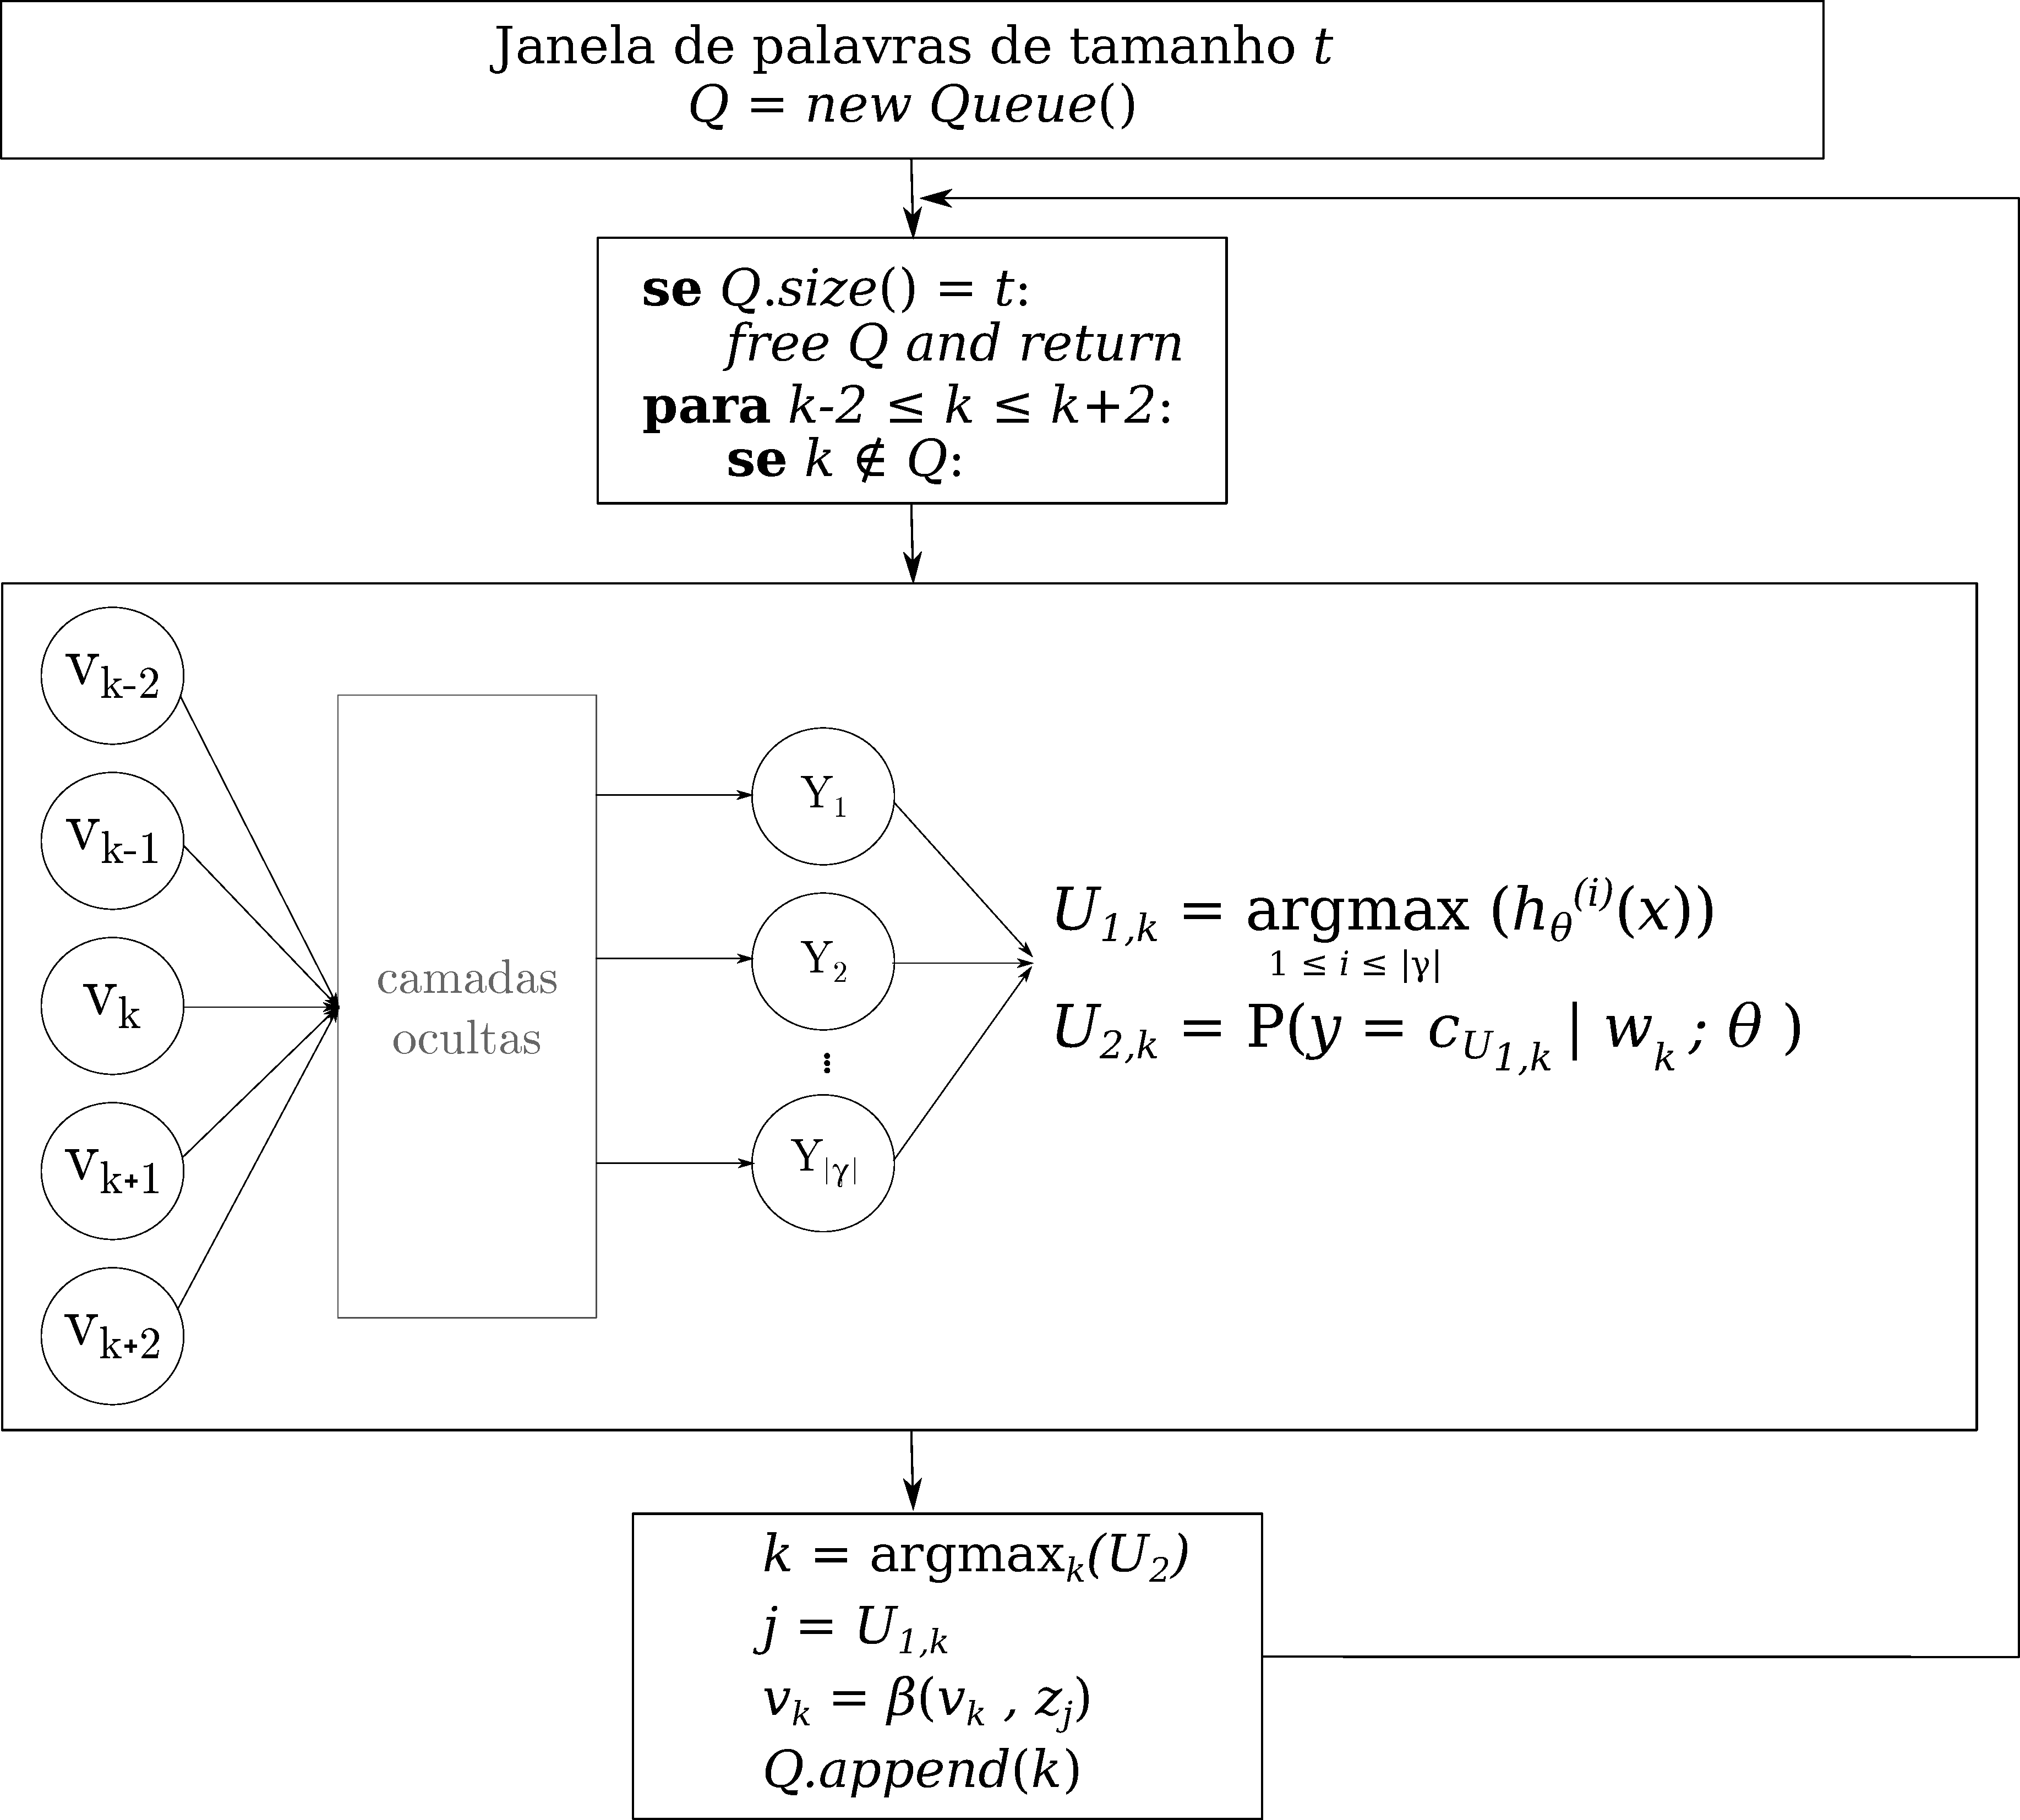
\includegraphics[scale=0.25]{img/neuralnetworkfinal_alg2.pdf}
%     \end{center}
% \end{figure}

% Para treinar a rede neural, será seguido uma estratégia de aprendizagem guiada por palavras mais fáceis \cite{shen2007guided}. A \autoref{fig:guidedlearning} exemplifica transições mais fáceis em uma frase, onde o peso mais baixo na aresta representa a ordem de execução. Na verdade, cada transição de um nodo para outro conta como uma nova etapa de treinamento. A \autoref{eq:pontuacaofinal} faz esse aprendizado guiado ao realizar a escolha da palavra mais fácil através da maximização das possibilidades que ainda não foram testadas dentro da janela de palavras.

% \begin{figure}[htb]
% 	  \caption{Grafo de transições de palavras mais fáceis}\label{fig:guidedlearning}
% 	  \begin{center}
% 	      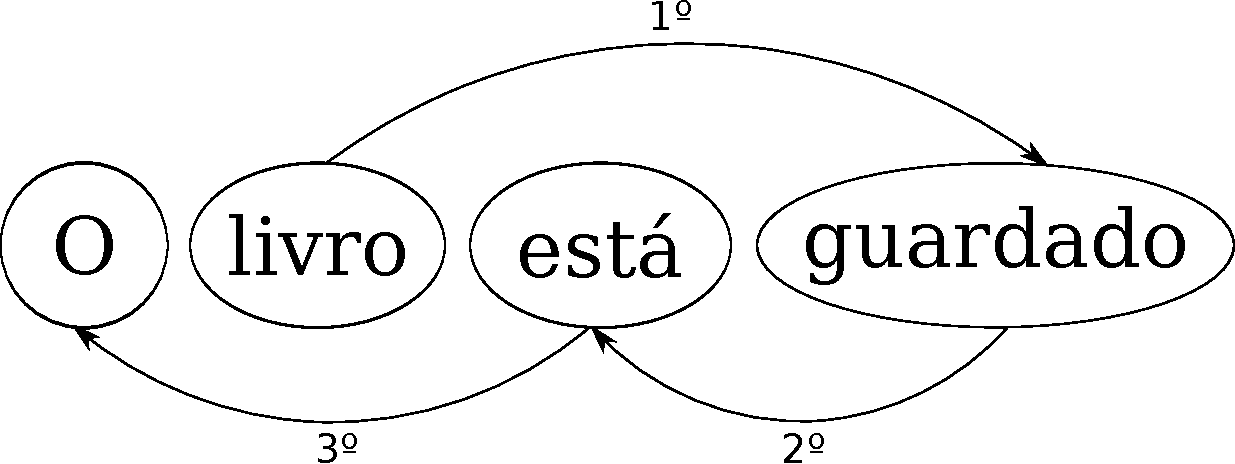
\includegraphics[scale=0.3]{img/guidedlearning.pdf}
% 	  \end{center}
% \end{figure}

% Treinar o modelo consiste em ajustar os pesos da rede neural, os valores das \textit{word embeddings} e as pontuações de transição. Após descobrir qual a classe gramatical mais provável para uma palavra $w_n$, o vetor da classe gramatical $z_c$ é composto com o vetor da própria palavra $v_n$ através de uma operação de soma. Essa composição é então armazenada no vetor da própria palavra, conforme mostrado abaixo. 

% \begin{equation} \label{eq:composicaovets}
% v_n = v_n + z_n
% \end{equation}

% Na rede neural da \autoref{fig:neuralnetworkfinal}, as camadas ocultas foram removidas da imagem para simplificar a visualização. A saída da rede neural é armazenada num conjunto temporário $U$, que tem duas listas. A primeira lista tem os índices da classe preditada para a palavra sendo analisada $w_k$, já a segunda lista contém as probabilidades da classe preditada ser da palavra $w_k$. Após isso, recupera-se qual a palavra que tem a maior probabilidade de ser classificada. O vetor da classe da palavra recuperada $z_j$ é composto com o vetor da palavra analisada $v_j$ através da \autoref{eq:composicaovets} e o processo se repete até que o conjunto $Q$ tenha tamanho $t$.

% Para treinar a rede neural, todos os ajustamentos são feitos em ordem de maximizar a seguinte equação:

% \begin{equation}
% \sum\limits_{(w_1^t,c_1^t) \in \phi} P(c_1^t|w_1^t,\theta) \nonumber \\
% \end{equation}

% Onde $\phi$ denota o conjunto dos pares de palavras e classes gramaticais. Computamos a probabilidade acima utilizando uma operação \textit{softmax} \cite{Bengio-et-al-2015-Book}:

% \begin{align}
% P(c_1^t|w_1^t,\theta) = &\ \dfrac{e^{S(w_1^t, c_1^t)}}{\sum\limits_{u_1^t \in \gamma^t} e^{S(w_1^t, u_1^t)}} \nonumber \nonumber \\
% log(P(c_1^t|w_1^t,\theta)) = &\ S(w_1^t, c_1^t) - log\Bigg(\sum\limits_{u_1^t \in \gamma^t} e^{S(w_1^t, u_1^t)} \Bigg) \nonumber
% \end{align}

% A função de custo pode ser definida como:

% \begin{equation} \label{eq:costfunctionfinalnn}
% J(\theta) = log\Bigg(\sum\limits_{u_1^t \in \gamma^t} e^{S(w_1^t, u_1^t)} \Bigg) - S(w_1^t, c_1^t)
% \end{equation}

% Onde, há princípio, ajustamos os pesos $\theta$ da rede utilizando o Gradiente Descendente sobre o primeiro termo da função de custo, porém vamos testar com outros algoritmos mais eficientes para essa tarefa, como o Gradiente Descendente Estocástico, Adagrad, Adadelta, etc. . 

% Também queremos maximizar o segundo termo da \autoref{eq:costfunctionfinalnn}. Para isso, seguimos \cite{fonseca2015evaluating} e realizamos um incremento nas pontuações de transição para cada palavra etiquetada em cada etapa do \textit{Backpropagation}, conforme mostrado na equação abaixo:

% \begin{equation}\label{eq:gradientsfinalnn}
% \frac{\partial J(\theta)}{\partial A_{c_{i-1}, c_{i}, c_{i+1}}} \text{ += } 1 \quad \forall i
% \end{equation}


% Além disso, incrementamos a função $s_c(v_k) \text{ += } 1$, onde $v_k$ representa a palavra no meio da janela sendo analisada.








\chapter{Modelo neural recorrente bidirecional}\label{modeloneuralrecorrentebidir}

Neste capítulo será explicado o outro modelo proposto para resolver o problema de \ac{pos} Tagging. Para isso, vamos falar primeiramente quais são os pré-processamentos feitos; depois vamos definir a arquitetura do modelo; explicar o algoritmo de treinamento e de predição; e por fim, comentar sobre a implementação do modelo.

Optamos por criar um modelo neural recorrente bidirecional, pois acreditamos que o uso de um contexto à direita pode influenciar na classificação, e que por usar \ac{gru}, a rede consegue aprender longas dependências.



\section{Pré-processamento}

Fizemos o mesmo pré-processamento que no modelo neural recursivo. Porém nesse modelo nós usamos um tamanho de janela grande para que a rede possa aprender longas dependências e ainda assim obter um contexto através das palavras vizinhas.


\section{Arquitetura}


A arquitetura do modelo neural recursivo implementado pode ser vista na \autoref{fig:recurrentmodel}.

\begin{figure}[!htb]
    \caption{Arquitetura da rede neural recorrente bidirecional}\label{fig:recurrentmodel}
    \begin{center}
        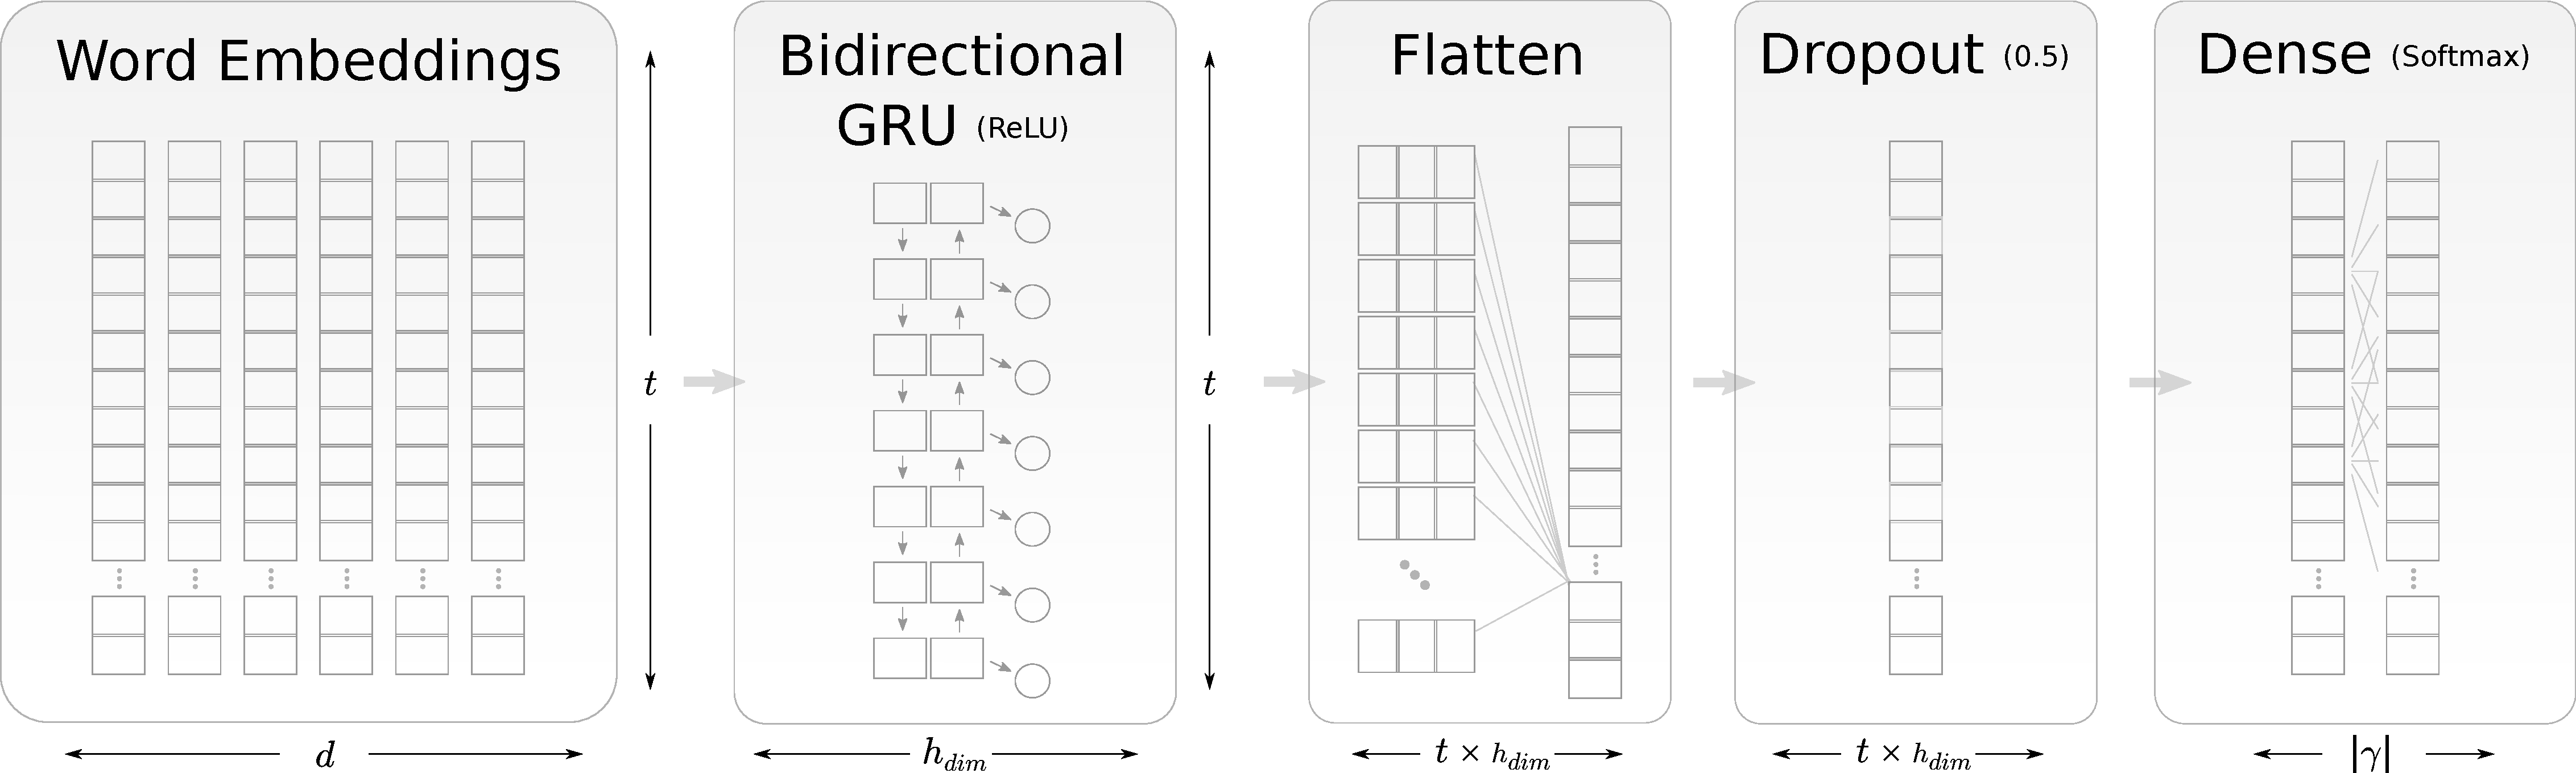
\includegraphics[scale=0.2]{img/recurrent_model_horizontal.pdf}
    \end{center}
\end{figure}


As diferenças na arquitetura do modelo recorrente bidirecional para o modelo recursivo é a inserção da \ac{gru} bidirecional e a retirada da camada de Embeddings para as etiquetas. Portanto, nessa seção vamos explicar apenas a camada recorrente bidirecional.

\subsection{GRU: camada recorrente bidirecional}

Conforme foi falado na \autoref{subsec:redesneuraisprofundas}, \ac{gru} é um tipo de rede neural que consegue aprender longas dependências entre termos numa sentença através da utilização de memória. No nosso caso, ela está recebendo uma janela de palavras $J_p$ de tamanho $t$. Para cada palavra nessa janela é produzida uma representação de tamanho $h_{dim}$. Desse modo, o formato da matriz de saída é $t \times h_{dim}$. 

Além disso, aplicamos a função de ativação \ac{relu} ao final da computação da \ac{gru}. A escolha dessa função de ativação foi feita de modo empírico.

\section{Treinamento}

Para treinar o modelo, simplesmente tentamos minimizar a função de custo da rede neural.

\subsection{Minimização da função de custo}

A função de custo escolhida foi a \textit{Categorial Cross-entropy} demonstrada na \autoref{eq:categorial_crossentropy}. Nós minimizamos essa função de custo utilizando o otimizador Adadelta, que também foi usado no modelo neural recursivo.


\section{Predição}

Para esse modelo pegamos a saída da rede para uma palavra como sendo a etiqueta prevista para ela.



\section{Implementação}

Implementamos esse modelo utilizando a mesma linguagem e as mesmas bibliotecas que foram usadas no modelo neural recursivo. O código da implementação da arquitetura, do treinamento e da predição podem ser vistos no \autoref{app:implementacaorecorrentebidir}.